
\chapter{Modeling} \label{ch:modeling}

To model the contact between the \gls{ee}'s tactile sensors, eight different categories exist as identified in~\cite{articulated-hands-force-control-and-kinematic-issues}. The three most common ones within the field of robotics~\cite[Chapter 37]{handbook-of-robotics} are \gls{pwof}, \gls{hf} and the \gls{sf} model as shown in \figref{fig:contact-models}. \medskip

\begin{figure}[h]
	\centering
	\begin{subfigure}[b]{0.3\textwidth}
		\centering
		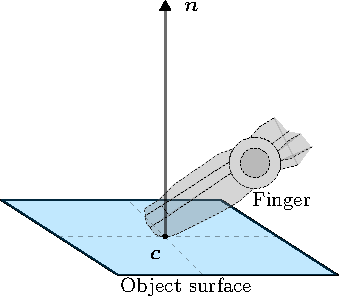
\includegraphics[width=\textwidth]{chapters/modeling/fig/contact-no-friction.pdf}
		\caption{\gls{pwof} in point \vec{c} with normal \vec{n}. \\\hspace{\textwidth} }
		\label{fig:pwof}
	\end{subfigure}
	\hfill
	\begin{subfigure}[b]{0.3\textwidth}
		\centering
		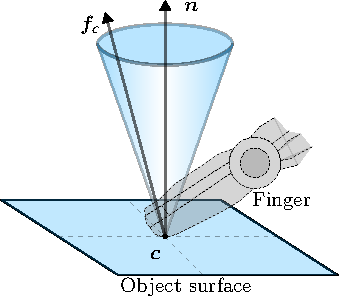
\includegraphics[width=\textwidth]{chapters/modeling/fig/hf.pdf}
		\caption{\gls{hf} in point \vec{c} with normal \vec{n} and contact force \mvar{\vec{f}_c}.}
		\label{fig:hf}
	\end{subfigure}
	\hfill
	\begin{subfigure}[b]{0.3\textwidth}
		\centering
		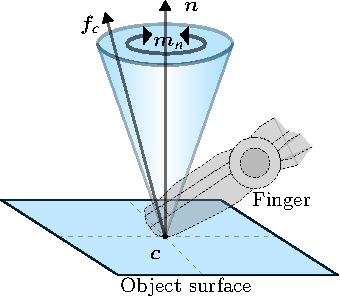
\includegraphics[width=\textwidth]{chapters/modeling/fig/sf.pdf}
		\caption{\gls{sf} in point \vec{c} with normal \vec{n}, contact force \mvar{\vec{f}_c} and friction moment \mvar{\vec{m}_n}.}
		\label{fig:sf}
	\end{subfigure}
	   \caption{The three most commonly used contact models.}
	   \label{fig:contact-models}
\end{figure}

% no friction
The \gls{pwof} model, as shown in \figref{fig:pwof}, can only represent forces along the surface normal \mvar{\vec{n}\inR{3}} at the point of contact \mvar{\vec{c}\inR{3}} and thus the model does not support surface deformations between the two contacting objects. This model is applied in cases where very little deformation is present, along with the contact having a friction coefficient approximately equal to zero~\cite[Chapter 38]{handbook-of-robotics}.\medskip


% Hard finger
The \gls{hf} model, as shown in \figref{fig:hf}, is representative when the friction between objects is significant, while the contact deformation is small enough to ignore friction moments and deformations~\cite[Chapter 38]{handbook-of-robotics}. To model the friction acting on the contact point a great number of methods exist, a common one being the Coulomb friction with different modifications depending on the use case~\cite{modelling-of-joint-friction-in-robotic-manipulators-with-gear-transmissions}. 
This model states that the frictional force acting on an object can be formulated as
%
\begin{equation}
	f_f = f_N \mu,
	\label{eq:coulomb-friction}
\end{equation}

with \mvar{f_f} being the magnitude of the Coulomb friction, \mvar{f_N} being the magnitude of the normal force in the point of contact and \mvar{\mu\in[0,1]} being the friction coefficient. One visualization of this linear relationship can be seen in the cones illustrated in \figref{fig:hf} and \figref{fig:sf}. These cones are referred to as friction cones, which for a hard finger model can be formulated as
%
\begin{equation} 
	\Chf = \left\{ \; f_c\; \middle|\; f_{t} \le \mu f_z,\; \mu f_z \ge 0 \; \right\} \qquad , \qquad f_t = \sqrt{f_x^2 + f_y^2}.
	\label{eq:hf}
\end{equation}
%
Here \mvar{f_c} is the magnitude of the contact force and \mvar{f_t} is the magnitude of the tangential force. \mvar{f_x}, \mvar{f_y} and \mvar{f_z} are the magnitudes of the \mvar{x}, \mvar{y} and \mvar{z} components of the contact force (\mvar{\vec{f}_c\inR{3}}) and \mvar{\mu} is the friction coefficient~\cite[Chapter 37]{handbook-of-robotics}. By applying a contact force that ensures the friction stays greater than the magnitude of the tangential force, neither object slips i.e. \mvar{f_z} must ensure that \mvar{f_z\mu} stays greater than \mvar{f_t} for the objects not to slip. Visually this is the case when the contact force \mvar{\vec{f}_c} stays within the friction cone, which enables a friction-based grasp type referred to as force closure. Specifically, force closure refers to when the composite wrench cone contains the entire wrench space so that any external wrench \vec{w_{\text{ext}}} on the body can be balanced by contact forces~\cite{modern-robotics-mechanics-planning-and-control}. A force that commonly contributes significantly to the external wrench, and thus to the tangential force, is gravity. \medskip

The \gls{sf} model, as shown in \figref{fig:sf}, is used to represent scenarios where both friction and surface deformations are significant. Due to deformations of the finger, an additional torsional moment about the contact normal will be present~\cite[Chapter 38]{handbook-of-robotics}. While an analytical formulation of the \gls{sf} relation depends on the pressure distribution inside the contact, and can only be derived for a limited number of special cases, the general case can be approximated using 
%
\begin{equation} 
	\Csf = \left\{ \; f_c \; \middle| \; f_t^2 + \frac{m_n^2}{e_n^2} \le \mu^2 P^2 \right\} \qquad , \qquad f_t = \sqrt{f_x^2 + f_y^2}.
	\label{eq:sf}
\end{equation}
This formulation forms a contact ellipsoid $\Csf$ which describes the relationship between the tangential force \mvar{\vec{f}_t\inR{3}} and friction moment \mvar{\vec{m}_n \inR{3}}. The friction parameters in this expression remain the same as for the friction cone, with the additional \mvar{m_n} being the magnitude of the frictional moment, \mvar{e_n} being the eccentricity parameter i.e. the height of the aforementioned ellipsoid and \mvar{P} being the magnitude of the pressure applied from the contact point along the contact normal \vec{n}~\cite{practical-force-motion-models-for-sliding-manipulation, soft-finger-model-with-adaptive-contact-geometry-for-grasping-and-manipulation-tasks}. \medskip

Based on the model categories described above, the most representative for this project's case, are the \gls{sf} models since these can provide information about the contact surface's shape, thus enabling the reconstruction of the contact shape from the application of a force distribution~\cite{contact-mechanics} i.e. the \gls{iep}. Additionally, these models support descriptions of friction which is crucial to manipulate objects in hand. Illustrations of the system as a \gls{sf} with friction cone, pressure distribution and the enabling of force closure can be seen in \figref{fig:friction-contact-distribution} and \figref{fig:force-closure-model} respectively.
%
\begin{center}
    \renewcommand{\arraystretch}{1.2}
    \begin{minipage}{.48\linewidth}
        \vspace{0pt}
        \centering
        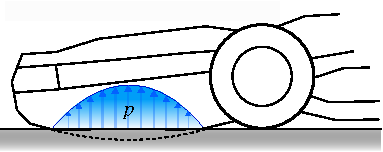
\includegraphics[width=.95\textwidth]{chapters/modeling/fig/contact-surface.pdf}%
        \vspace{0.6cm}
        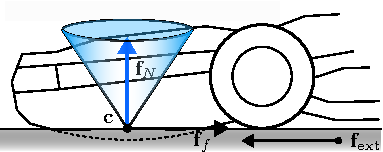
\includegraphics[width=.95\textwidth]{chapters/modeling/fig/friction-cone-schematic.pdf}%
    \end{minipage}%
    \hfill%
    \begin{minipage}{.48\linewidth}
        \vspace{0pt}
        \centering
        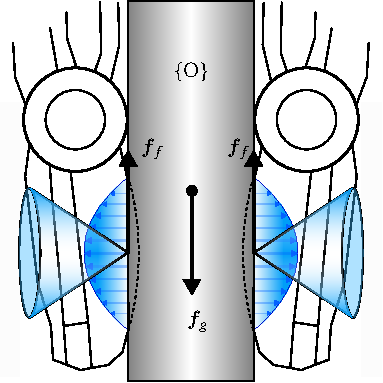
\includegraphics[width=.95\textwidth]{chapters/modeling/fig/force-closure-schematic.pdf}
    \end{minipage}%
    %    
    \vspace{15pt}
    %
    \begin{minipage}[t]{.48\linewidth}
        \vspace{0pt}
        \captionsetup{type=figure}
        \captionof{figure}{The pressure distribution \mvar{p} and friction cone of a \gls{sf} model experiencing an external force \mvar{\vec{f}_{\text{ext}}}.}
        \label{fig:friction-contact-distribution}
    \end{minipage}%
    \hfill%
    \begin{minipage}[t]{.48\linewidth}
        \vspace{0pt}
        \captionsetup{type=figure}
        \captionof{figure}{the pressure distribution and friction cone causing force closure to prevent the object \robframe{O} from falling due to the gravitational force \mvar{\vec{f}_g}.}
        \label{fig:force-closure-model}
    \end{minipage}%
\end{center}
When modeling the kinematics of an anthropomorphic gripper with frame \mvar{\robframe{H}\inR{4\times 4}} in world frame \mvar{\robframe{W}\inR{4\times 4}} interacting with an object with frame \mvar{\robframe{O}\inR{4\times 4}} the relevant parameters must be addressed. In this system the object with position \mvar{\vec{p}\inR{3}} and pose \mvar{\vec{u}\inR{6}}, with the orientation either being represented as a four-dimensional quaternion or a three-dimensional Euler angle, makes contact with the gripper in points \mvar{\vec{c}_i\inR{3}}. These contact points have frames \mvar{\robframe{C}_i\inR{4 \times 4}} with axes \mvar{\rlist{\vec{n}_i,\vec{t}_i,\vec{o}_i}\subset \R^{3}}, where \mvar{\vec{n}_i\inR{3}} points perpendicular to the contact plain towards the object, while the remaining are contained within the contact plane. For each of these parameters \mvar{i=1,2,\ldots,n_c}, where \mvar{n_c} is the number of contact points. The twist of \robframe{O} described in \robframe{W} is denoted \mvar{\vec{\nu} = \rvec{\vec{v}^\T \vsep \vec{\omega}^\T}^\T\inR{6}} while the non-contact wrench i.e. the wrench caused by external forces such as collisions with the environment and gravity, is \mvar{\vec{w} = \rvec{\vec{f}^\T \vsep \vec{m}^\T}^\T\inR{6}}. The gripper's state is described in terms of its joints, of which it has \mvar{n_q}, named \mvar{\vec{q} = \rvec{q_1  \vsep q_2  \vsep \dots  \vsep q_{n_q}}^\T\in\R^{n_q}} each of which is revolute and can exert a torque \mvar{\vec{\tau} = \rvec{\tau_1  \vsep\tau_2  \vsep\dots  \vsep\tau_{n_q} \vsep}^\T\in\R^{n_q}}. These parameters can be seen illustrated in \figref{fig:sys-schematic} showing the system model. While only a single finger here is illustrated the naming conventions and representations simply scale to all the \gls{ee}'s \gls{dof}s.
%
\begin{figure}[h]
	\begin{small}
		\begin{center}
			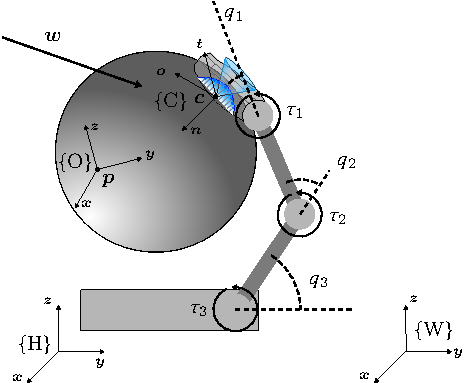
\includegraphics[width=0.6\textwidth]{chapters/modeling/fig/sys-schematic-reversed-crop.pdf}
		\end{center}
		\caption{The model of the system representation for this project.}
		\label{fig:sys-schematic}
	\end{small}
\end{figure}

In this system, the twists and wrenches of a contact point \mvar{\vec{c}_i} on the object and hand, given in contact frame \mvar{\robframe{C}_i} is referred to as \mvar{\vec{\nu}_{i,\xi}\inR{6}} and \mvar{\vec{w}_{i,\xi}\inR{6}}, with \mvar{\xi = \rlist{\text{obj}, \text{hnd}}}. Given multiple contact points, complete vectors of twist and wrench can be expressed by appending each contact point's twist and wrench vector. These contain all twists and wrenches of the grasp, one for the object and one for the hand. These vectors are referred to as 
%
\begin{equation}
	\vec{\nu}_{c,\xi} = \rvec{\vec{\nu}_{1,\xi}^\T \vsep \vec{\nu}_{2,\xi}^\T \vsep \ldots \vsep \vec{\nu}_{n_c,\xi}^\T}^\T \inR{6\cdot n_c}
	\label{eq:complete-twists}
\end{equation}
%
and
\begin{equation}
	\vec{w}_{c,\xi} = \rvec{\vec{w}_{1,\xi}^\T \vsep \vec{w}_{2,\xi}^\T \vsep \ldots \vsep \vec{w}_{n_c,\xi}^\T}^\T \inR{6\cdot n_c}
	\label{eq:complete-wrenches}
\end{equation}
%
respectively. \medskip

These definitions are used to describe and analyze the kinematics of grasping and the parameters involved in holding and manipulating objects in hand, also referred to as \gls{gk}. Within \gls{gk} two matrices are of special interest: the grasping matrix \mat{G} and the hand Jacobian \mat{J}. The grasping matrix describes the transformation between the twist or wrench of the object in world frame \robframe{W} to the twists or wrenches of the object in contact frames \mvar{ \robframe{C}_i}. The grasp matrix thus can be expressed as
%
\begin{equation}
	\mat{G} = \rvec{ \mat{G}_1 \vsep \mat{G}_2 \vsep \mat{G}_3 \vsep \cdots \vsep \mat{G}_{n_c}},
	\label{eq:grasp-matrix-def}
\end{equation}
%
where \mvar{\mat{G}_i \inR{6\times 6}} describes the transformation from \robframe{W} to the individual \mvar{\robframe{C}_i}, and thus \mvar{\mat{G}\inR{6\times 6\cdot n_c}} describes the transformations for all contact points. Using this grasp matrix, the object wrench and twist can be computed in all contact frames as
%
\begin{equation}
	\vec{\nu}_{c,\text{obj}} =  \mat{G}^\T \vec{\nu} \mspa \mand \mspa \vec{w}_{c,\text{obj}} =  \mat{G}^\T \vec{w}.
	\label{eq:grasp-matrix-twist}
\end{equation}
%
While the grasp matrix describes the transformation from \robframe{W} to object contact frames, the hand Jacobian relates the joint velocities and torques to the contact twists and wrenches on the hand. The hand Jacobian can thus be expressed as 
%
\begin{equation}
	\mat{J} = \rvec{ \mat{J}_1^\T \vsep \mat{J}_2^\T \vsep \mat{J}_3^\T \vsep \cdots \vsep \mat{J}_{n_c}^\T}^\T,
	\label{eq:hand-jacobian-matrix}
\end{equation}
%
for all contact points. Here \mvar{\mat{J}_i \inR{6 \times n_q} \mfor i = 1,2,\ldots,n_c} are the individual contact points' hand Jacobians and thus \mvar{\mat{J}\inR{6 \cdot n_c \times n_q}} is the complete. Using the complete hand Jacobian, the contact twists and wrenches on the hand can be related to the joint velocities and torques as
% 
\begin{equation}
	\vec{\nu}_{c,\text{hnd}} = \mat{J} \dot{\vec{q}} \mspa \mand \mspa \vec{\tau} = \mat{J}^\T \vec{w}_{c,\text{hnd}}.
	\label{eq:hand-jacobian-velocity}
\end{equation}

The modeling described above will enable the use of methods for solving the presented problems. These methods will be described in \chapref{ch:1-tactile-perception}.
